\documentclass{article}
\usepackage[utf8]{inputenc}

\title{System Operations Lab \newline Assignment}
\author{Vrishti Jain}
\date{16 Oct 2018}
\newpage
\usepackage{graphicx}
\usepackage{enumitem}
\newlist{steps}{enumerate}{1}
\setlist[steps, 1]{label = Step \arabic*:}
\begin{document}


\maketitle

\section{Installation with creation of file system using
fdisk (manual) with at least one logical partition}

We will first list all the existing partitions. Then add a partition with the help of fdisk GUI. Then again list the partitions.
\newline
\newline
\textbf{Steps to Follow} 
\newline
Step 1 : List the partitions
\newline

\begin{center}
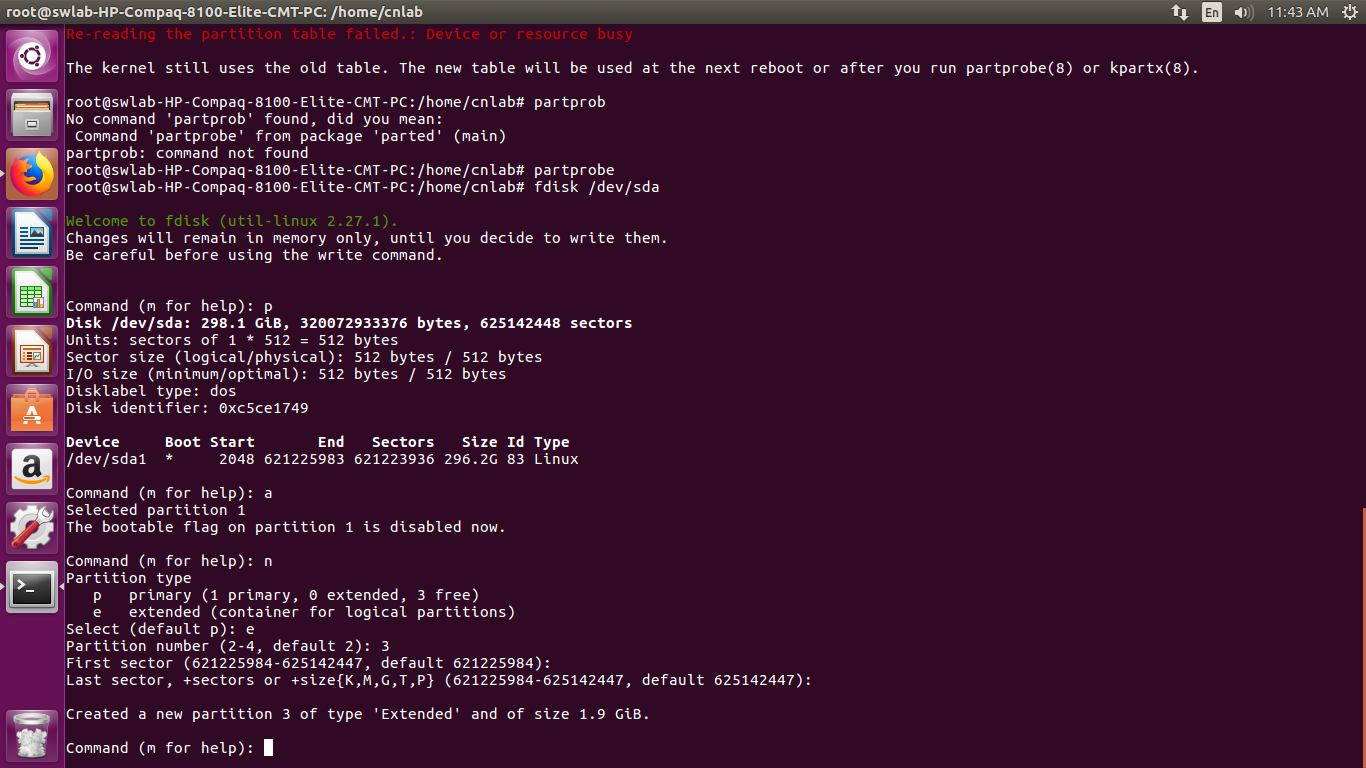
\includegraphics[scale=0.2]{partison1.png}
\end{center}
Step 2: Adding a new partition
\newline
\begin{center}
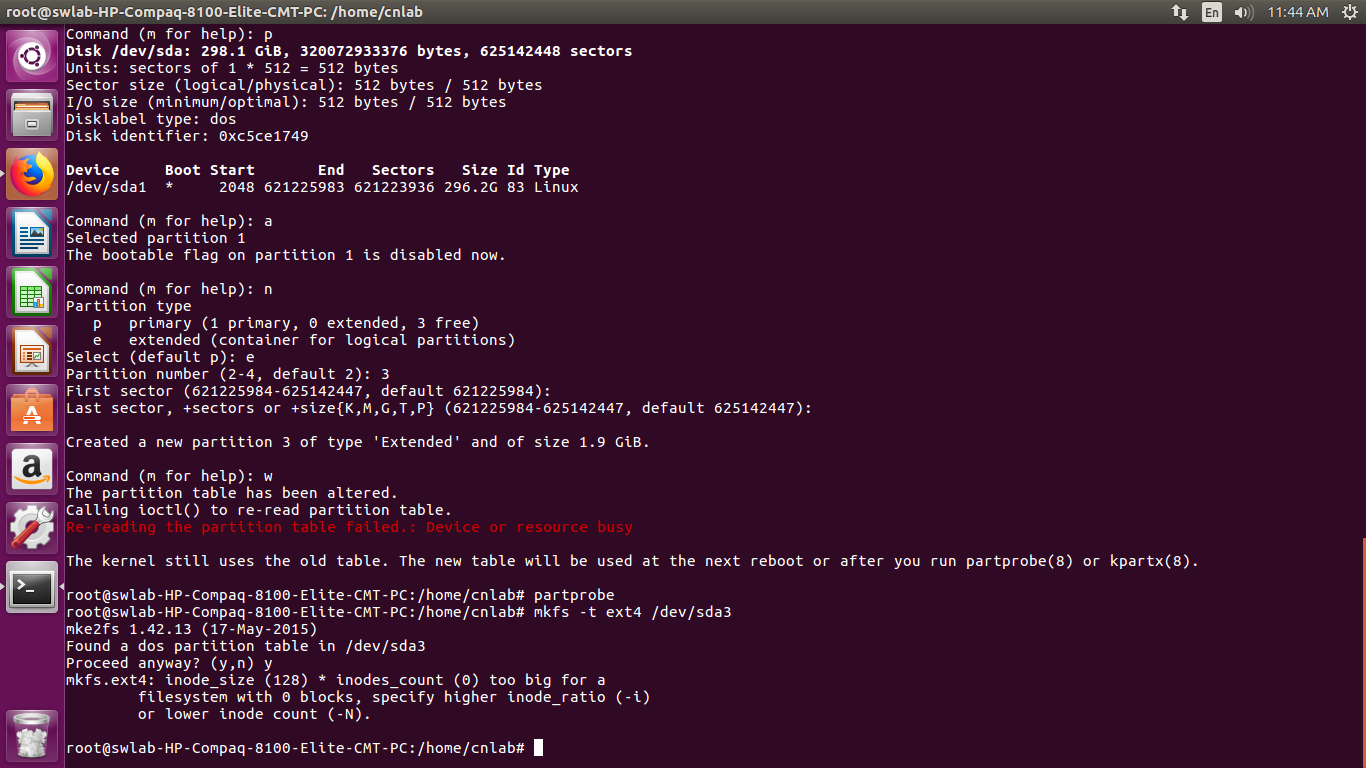
\includegraphics[scale=0.2]{PARTISON2.png}
\end{center}
Step 3 : List partitions again to view the new added partition

\section{Root Password change using boot loader options}
Since everything happens during the boot time. It's unable to click screen shots. So I would just lay out the steps of changing the password during boot.
\newline\newline
\textbf{Steps to Follow}
\begin{steps}
\item Restart the computer
\item Open the Grub GUI during boot up.
\item Highlight the OS in which you want to change the root password.
\item Press E to edit that OS.
\item Edit the line starting with linux. By appending \textbf{rw init=/bin/bash}
\item Now you will be taken to the root shell.
\item Run command \textbf{passwd}. and change the passwd
\item Run \textbf{exec=/sbin/init}.
\newline
\begin{center}
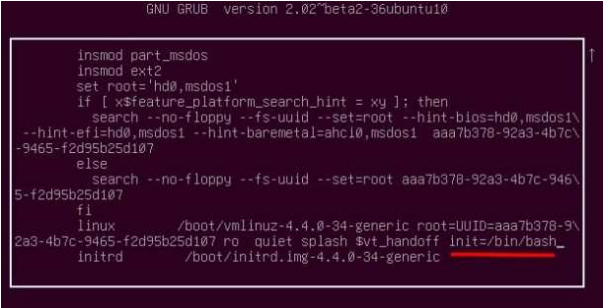
\includegraphics[scale=1]{pass.PNG}
\newpage
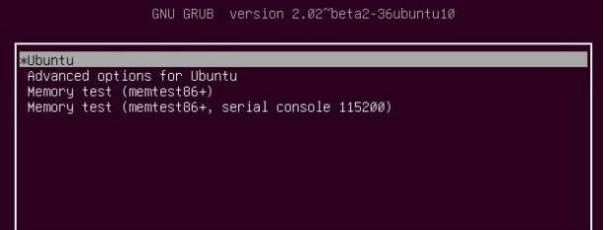
\includegraphics[scale=1]{partison3.PNG}
\end{center}
\newpage
\end{steps}
\newpage
\section{Directory creation in which all can write but only owner can delete files.}

This can be done via sticky bit. This helps only the owner of the files to delete from that particular folder. No one else can delete the files in that folder.
\newline\newline
\textbf{Steps to Follow}
\newline\newline
Step 1 : Making a folder named \textbf{newFold}. Creating a file named \textbf{file.txt}.\newline

Step 2 : Switching to another user. Then trying to delete this file.\newline
\begin{center}
    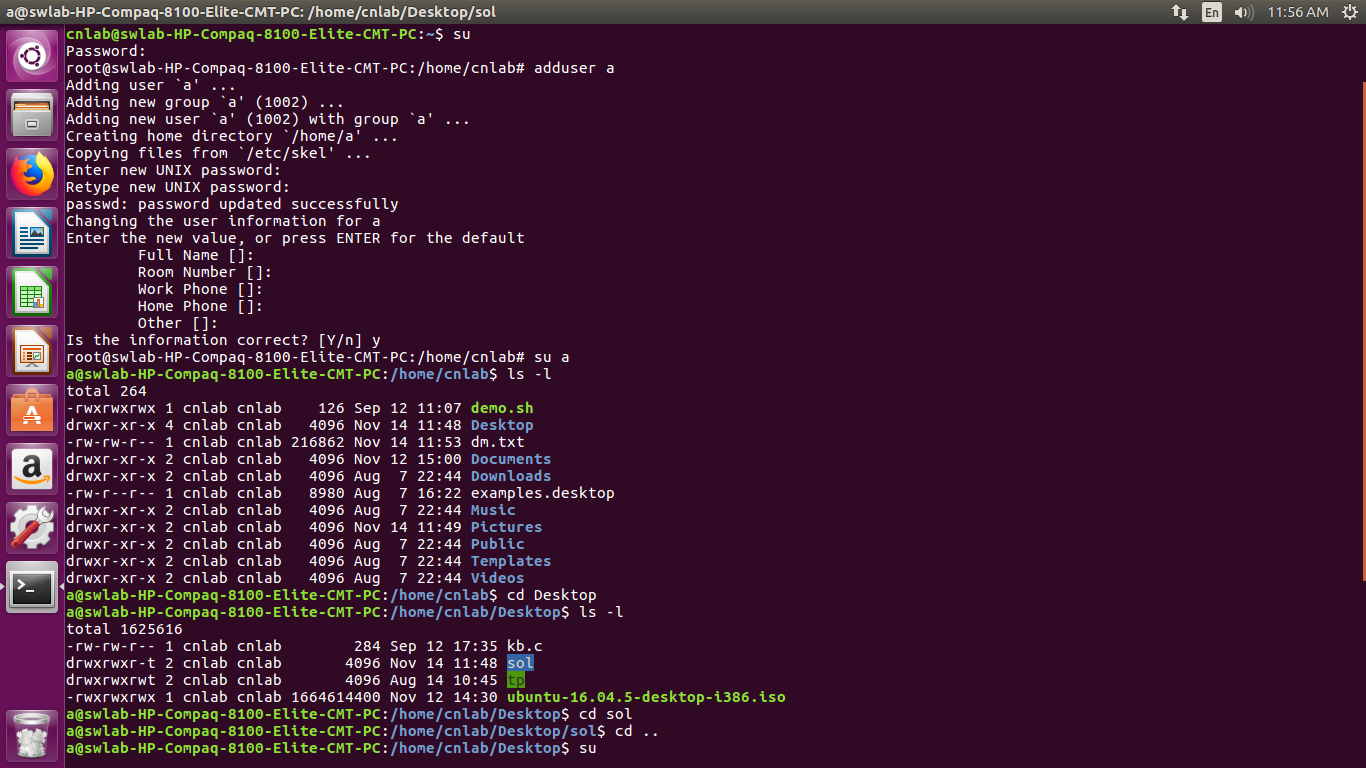
\includegraphics[scale=0.2]{sticky2.png}
    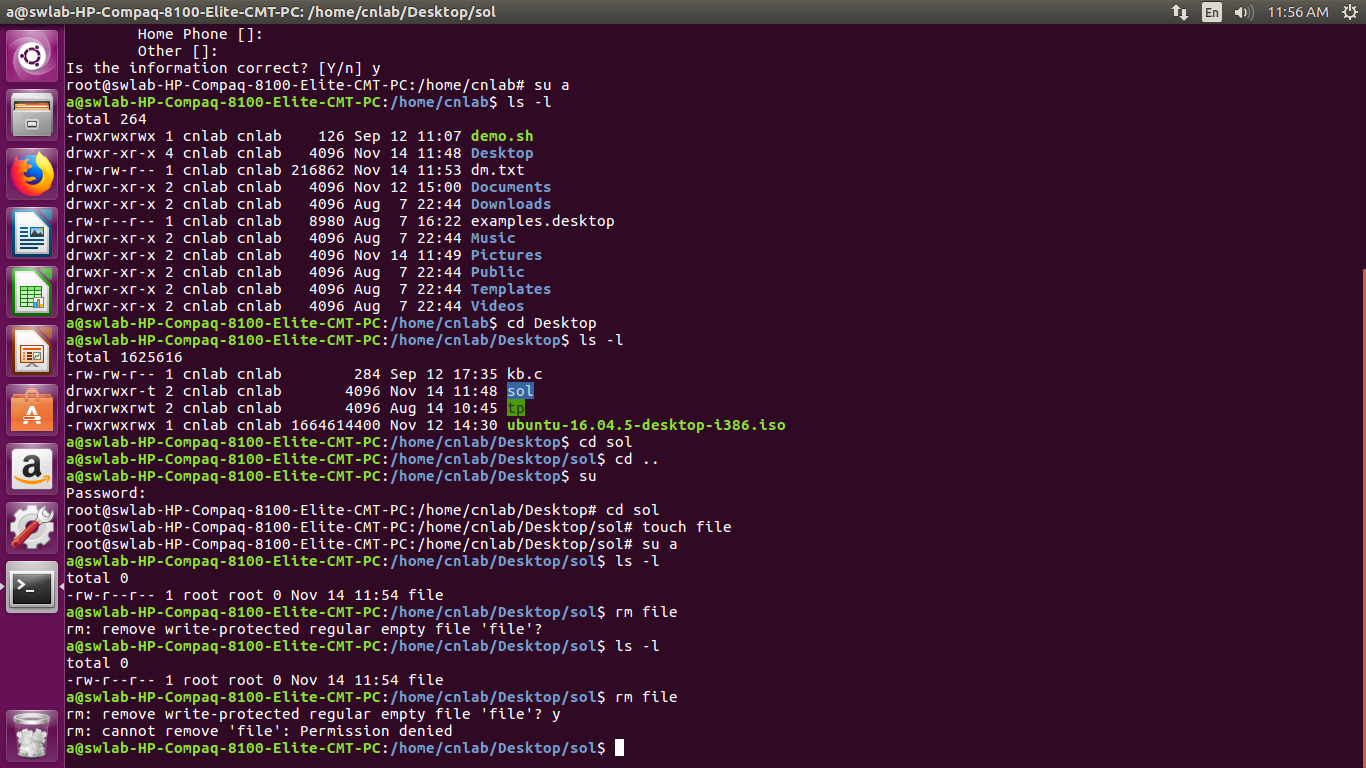
\includegraphics[scale=0.2]{sticky3.png}
\end{center}
\newpage
\section{Write a cron job to remote power up a system in a LAN}
For this assignment we need to have the MAC address of the other system on the LAN for which we have to perform this cron job.
\newline
\newline
\textbf{Steps to Follow}
\newline
Step 1 : First open the file \textbf{/etc/crontab}\newline
\begin{center}
    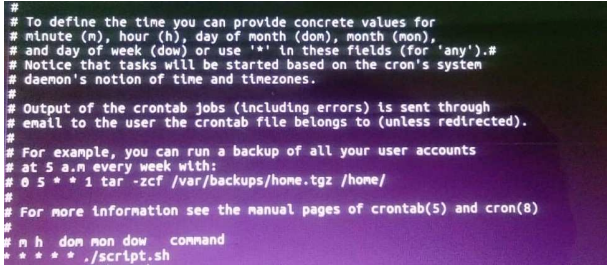
\includegraphics[scale=1]{cron1.PNG}
\end{center}
Step 2 : Edit the file.\newline
\begin{center}
    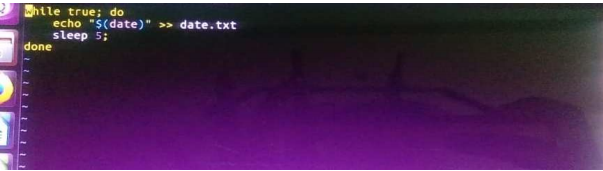
\includegraphics[scale=1]{cron2.PNG}
\end{center}
\newpage
\section{Write a cron job to remotely shutdown a Linux system.}
For this assignment we need to have the MAC address of the other system on the LAN for which we have to perform this cron job.
\newline
\newline
\textbf{Steps to Follow}
\newline
Step 1 : First open the file \textbf{/etc/crontab}\newline
\begin{center}
    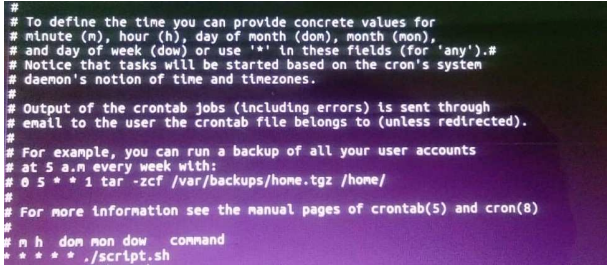
\includegraphics[scale=1]{cron1.PNG}
\end{center}
Step 2 : Edit the file.\newline
\begin{center}
    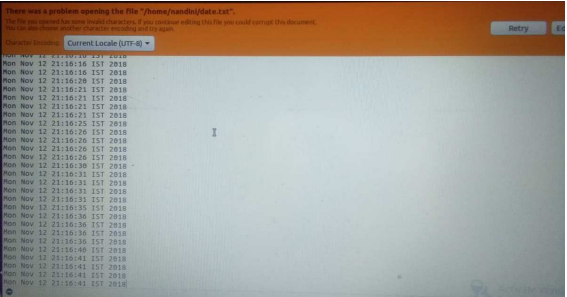
\includegraphics[scale=1]{cron3.PNG}
\end{center}
\newpage


\section{In Git account add new project and shows commits.}
For this assignment we need to have an github account and create an repository.
\newline
\newline
\textbf{Steps to Follow}
\newline
Step 1 : Create a repository. \textbf{/etc/crontab}\newline
\begin{center}
    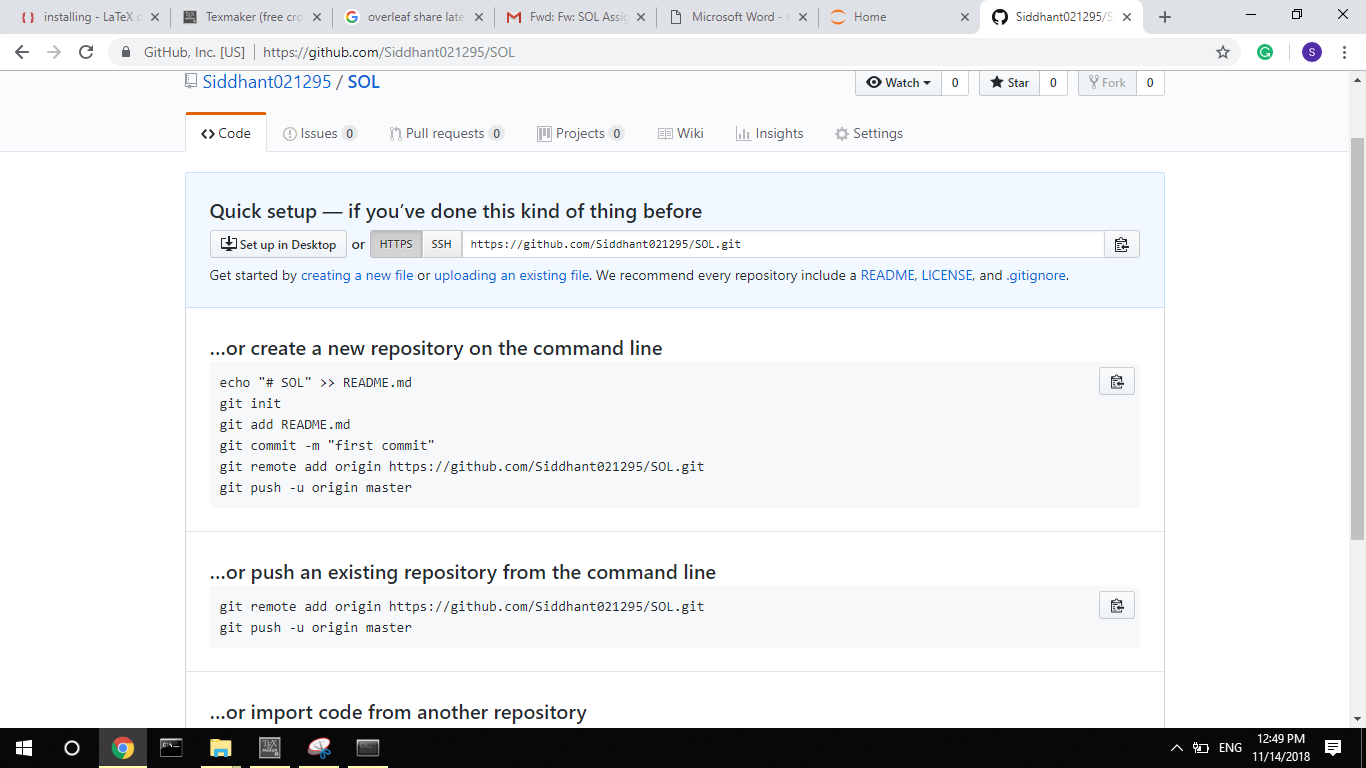
\includegraphics[scale=0.2]{git1.png}
\end{center}
Step 2 : Create a folder and run git init.\newline
\begin{center}
    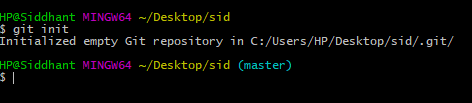
\includegraphics[scale=1]{git2.png}
\end{center}
Step 3 : Create different file you want to commit and \newline
\begin{center}
    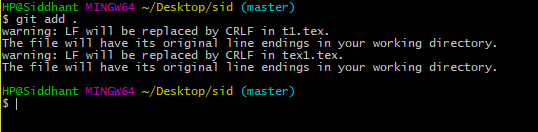
\includegraphics[scale=1]{git3.png}
\end{center}
\newpage
Step 4 : Add files to the staging area. Run git add . \newline
\begin{center}
    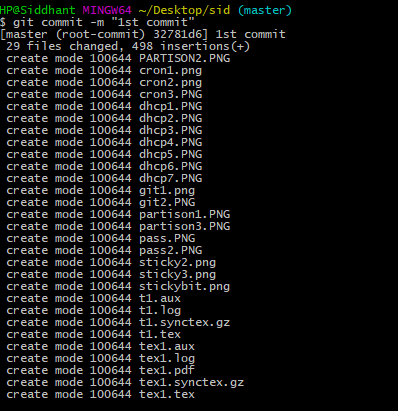
\includegraphics[scale=1]{git4.png}
\end{center}
\newpage
Step 5 : Commit the changes. Run git commit -m "message" . \newline
\begin{center}
    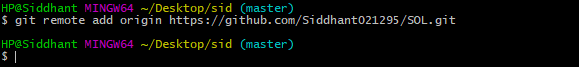
\includegraphics[scale=1]{git5.png}
\end{center}
\newpage
\end{document}
